\documentclass{article}
\usepackage[utf8]{inputenc}
\usepackage{subfig}
\usepackage{amsmath}

\usepackage{graphicx}
\usepackage[a3paper, landscape, margin=0.5cm]{geometry}

\thispagestyle{empty}
% \renewcommand{\thesubfigure}{\roman{subfigure}}
\begin{document}

\begin{figure}[t]
        \centering
        \subfloat[profile (FF)]{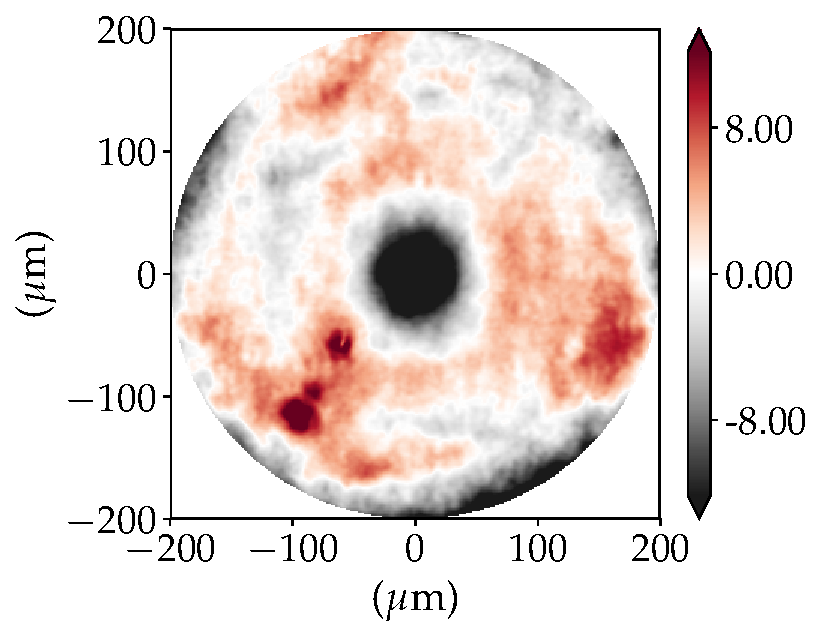
\includegraphics[height=3.5cm]{figures/ch05/CDnFF_LF_HH/CDn_individual_12p39842keV_n_10.0_lsp2p0mm_cpp2p0mm_phase_figure_errors_FF.pdf}}\hspace{0.1cm}
        \subfloat[vertical caustics]{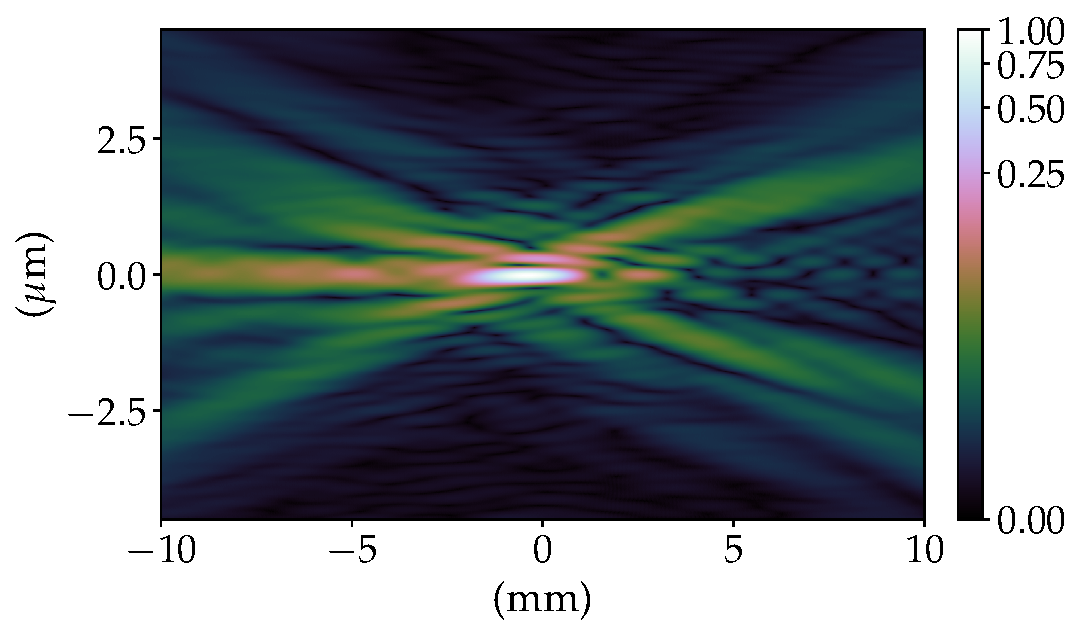
\includegraphics[height=3.4cm]{figures/ch05/CDnFF_LF_HH/Be_CDn_8p0keV_d0p0mm_n10_intensity_cstc_Y_cstc_2D.pdf}}\hspace{0.1cm}
        \subfloat[PSF phase (rad)]{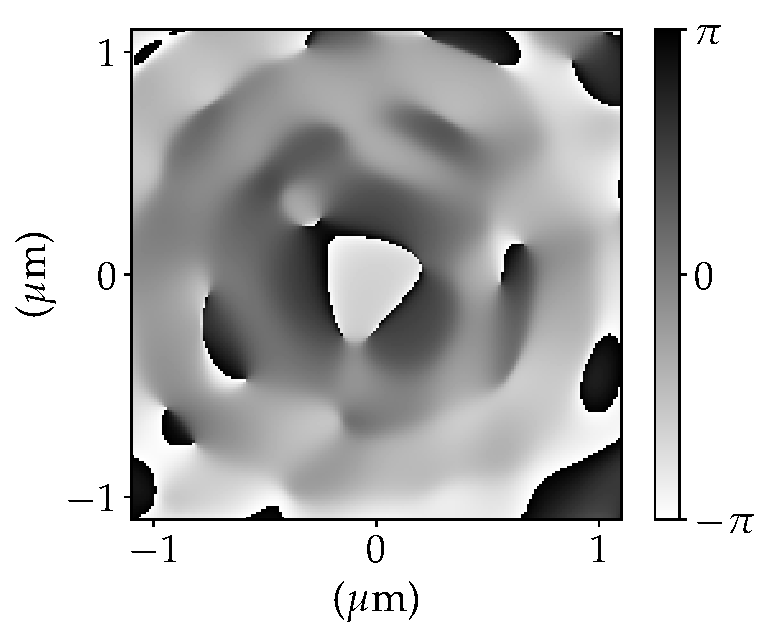
\includegraphics[height=3.5cm]{figures/ch05/CDnFF_LF_HH/Be_CDn_8p0keV_d0p0mm_n10_phase_phase_2D.pdf}}\hspace{0.1cm}
        \subfloat[PSF intensity]{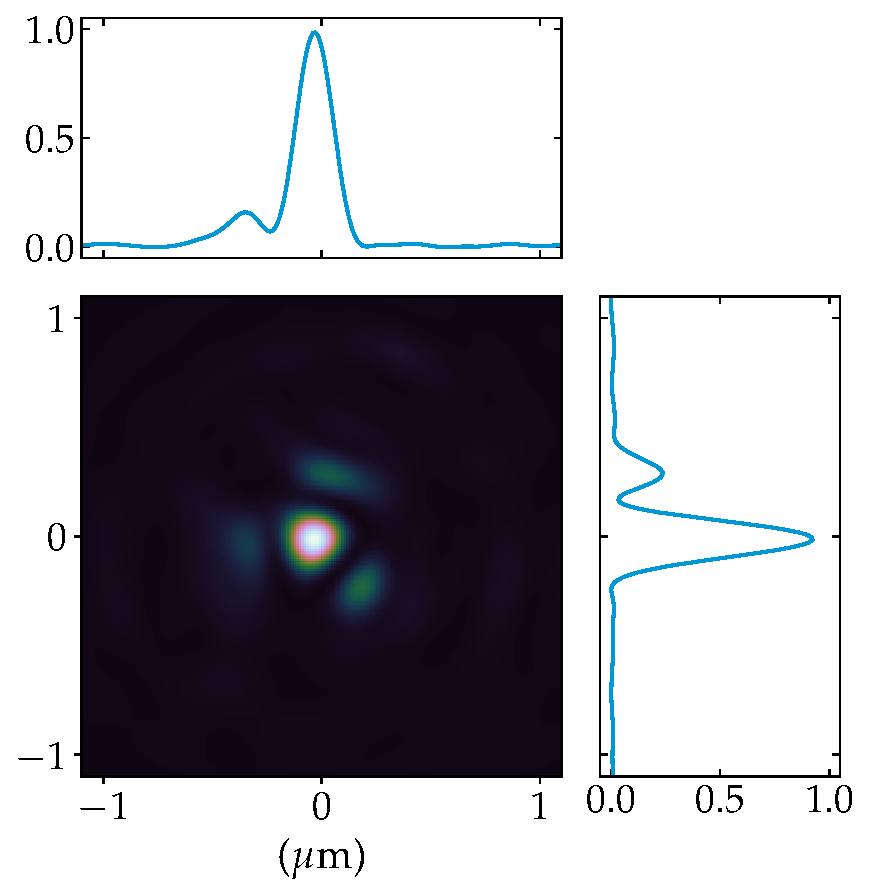
\includegraphics[height=5cm]{figures/ch05/CDnFF_LF_HH/Be_CDn_8p0keV_d0p0mm_n10_intensity_intensity_2D.pdf}}\hspace{0.1cm}
        \caption*{figure errors}\vspace{0.3cm}\setcounter{subfigure}{0}
        \subfloat[profile (LF)]{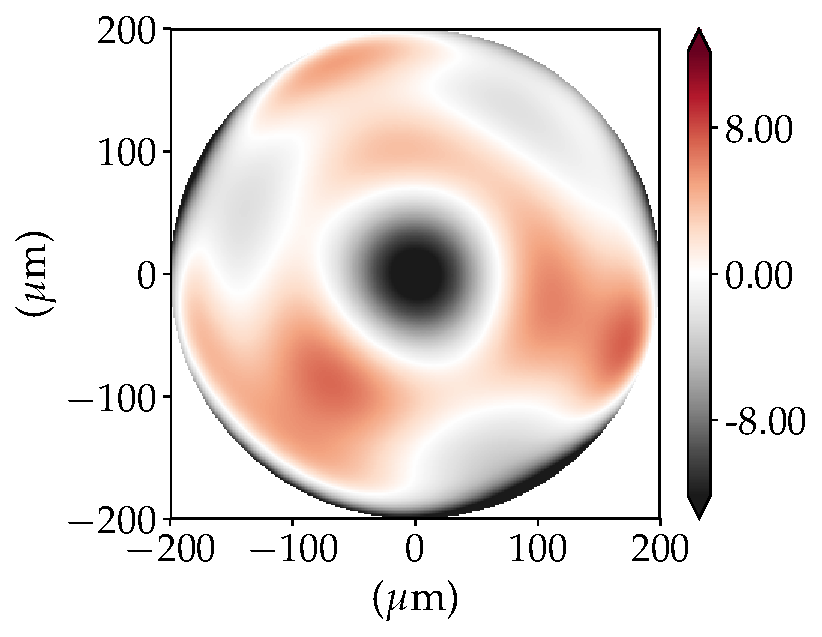
\includegraphics[height=3.5cm]{figures/ch05/CDnFF_LF_HH/CDn_individual_12p39842keV_n_10.0_lsp2p0mm_cpp2p0mm_phase_figure_errors_LF.pdf}}\hspace{0.1cm}
        \subfloat[vertical caustics]{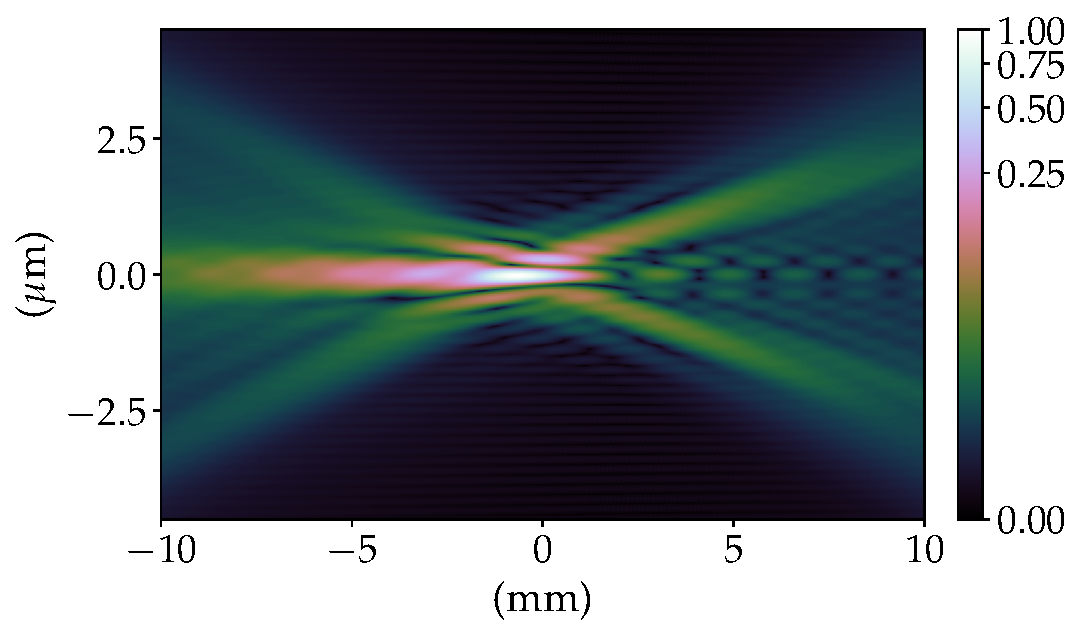
\includegraphics[height=3.4cm]{figures/ch05/CDnFF_LF_HH/Be_CDn_LF_8p0keV_d0p0mm_n10_intensity_cstc_Y_cstc_2D.pdf}}\hspace{0.1cm}
        \subfloat[PSF phase (rad)]{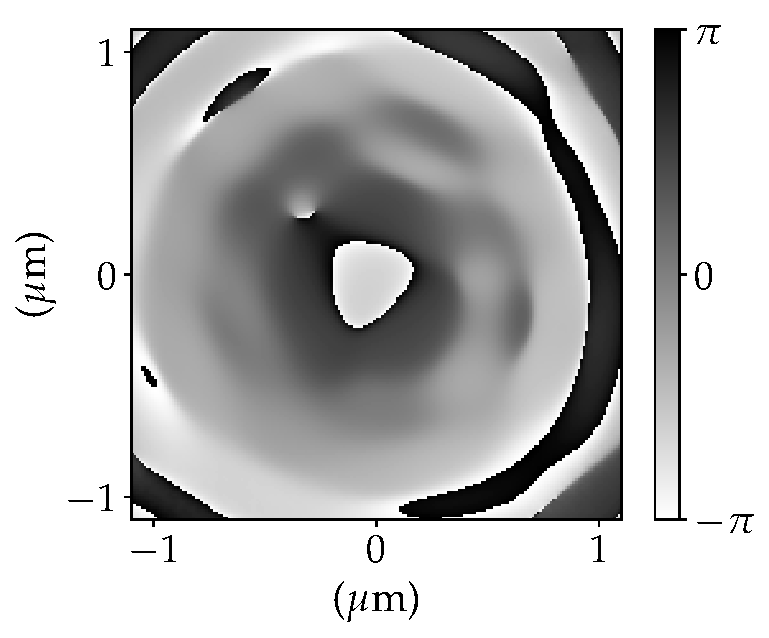
\includegraphics[height=3.5cm]{figures/ch05/CDnFF_LF_HH/Be_CDn_LF_8p0keV_d0p0mm_n10_phase_phase_2D.pdf}}\hspace{0.1cm}
        \subfloat[PSF intensity]{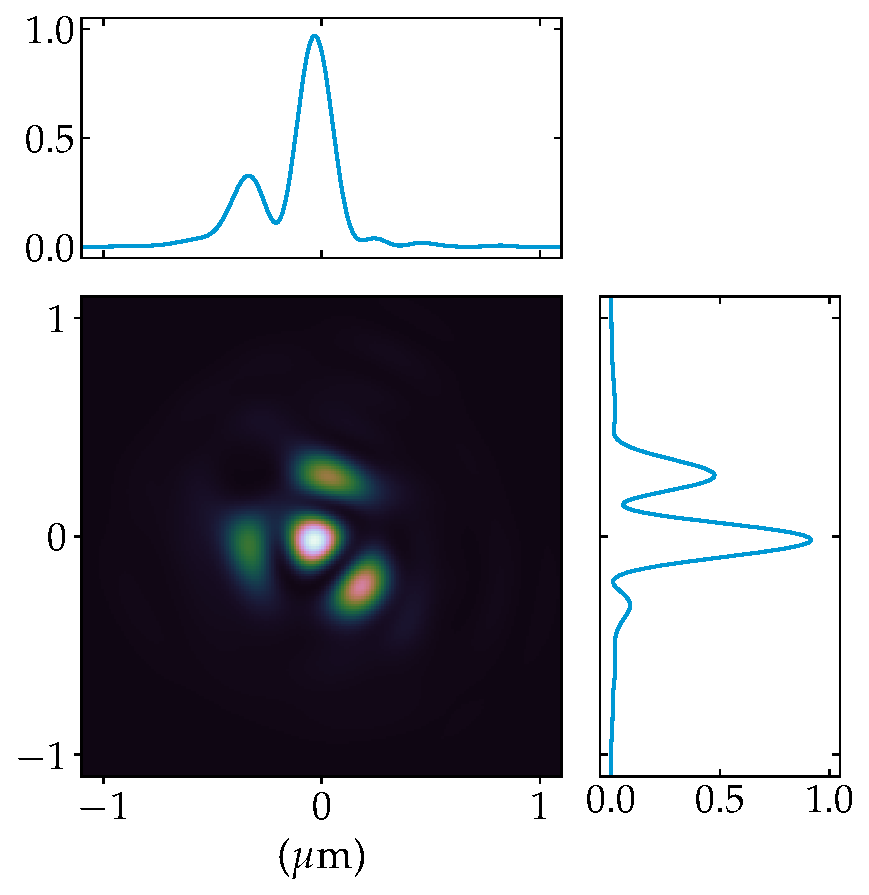
\includegraphics[height=5cm]{figures/ch05/CDnFF_LF_HH/Be_CDn_LF_8p0keV_d0p0mm_n10_intensity_intensity_2D.pdf}}\hspace{0.1cm}
        \caption*{polynomial fit profile }\vspace{0.3cm}\setcounter{subfigure}{0}
        \subfloat[profile (HF)]{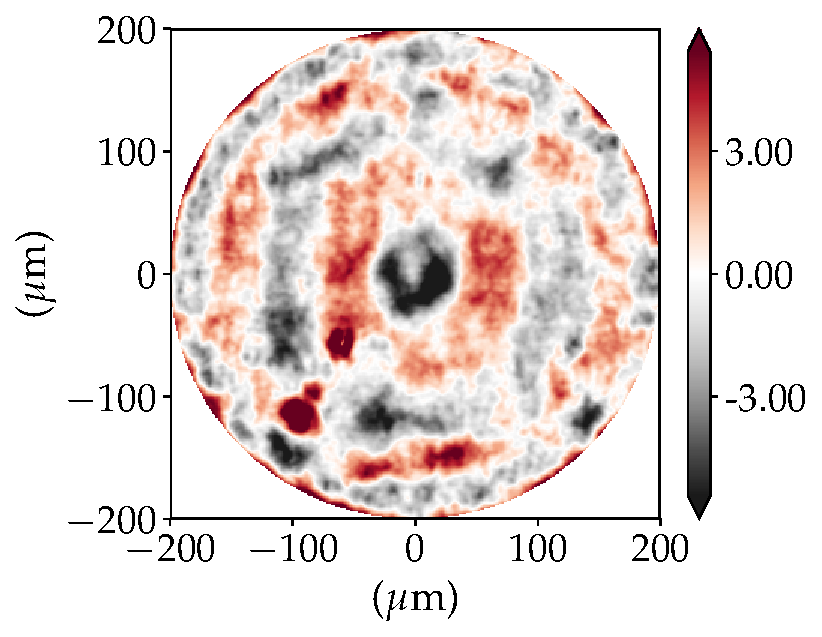
\includegraphics[height=3.5cm]{figures/ch05/CDnFF_LF_HH/CDn_individual_12p39842keV_n_10.0_lsp2p0mm_cpp2p0mm_phase_figure_errors_HF.pdf}}\hspace{0.1cm}
        \subfloat[vertical caustics]{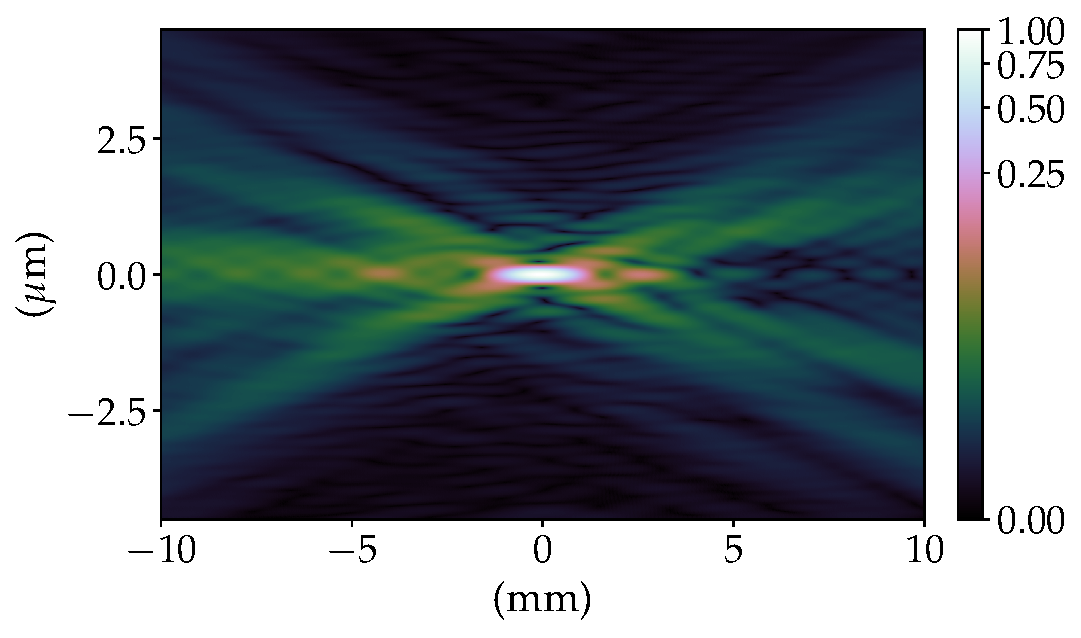
\includegraphics[height=3.4cm]{figures/ch05/CDnFF_LF_HH/Be_CDn_HF_8p0keV_d0p0mm_n10_intensity_cstc_Y_cstc_2D.pdf}}\hspace{0.1cm}
        \subfloat[PSF phase (rad)]{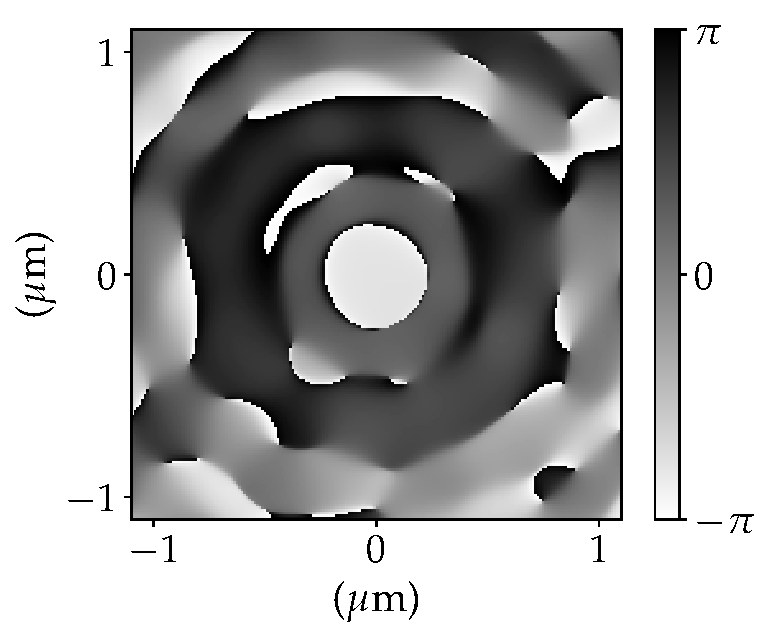
\includegraphics[height=3.5cm]{figures/ch05/CDnFF_LF_HH/Be_CDn_HF_8p0keV_d0p0mm_n10_phase_phase_2D.pdf}}\hspace{0.1cm}
        \subfloat[PSF intensity]{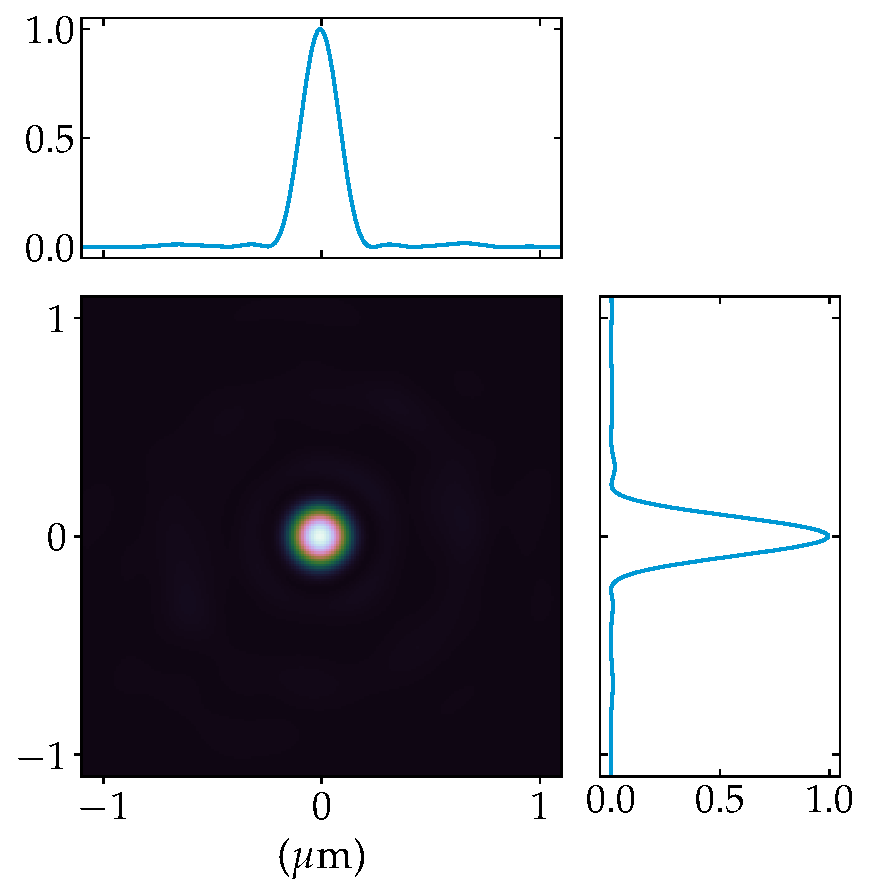
\includegraphics[height=5cm]{figures/ch05/CDnFF_LF_HH/Be_CDn_HF_8p0keV_d0p0mm_n10_intensity_intensity_2D.pdf}}\hspace{0.1cm}
        \caption*{residue profile}\vspace{0.3cm}
        \subfloat[Strehl ratio]{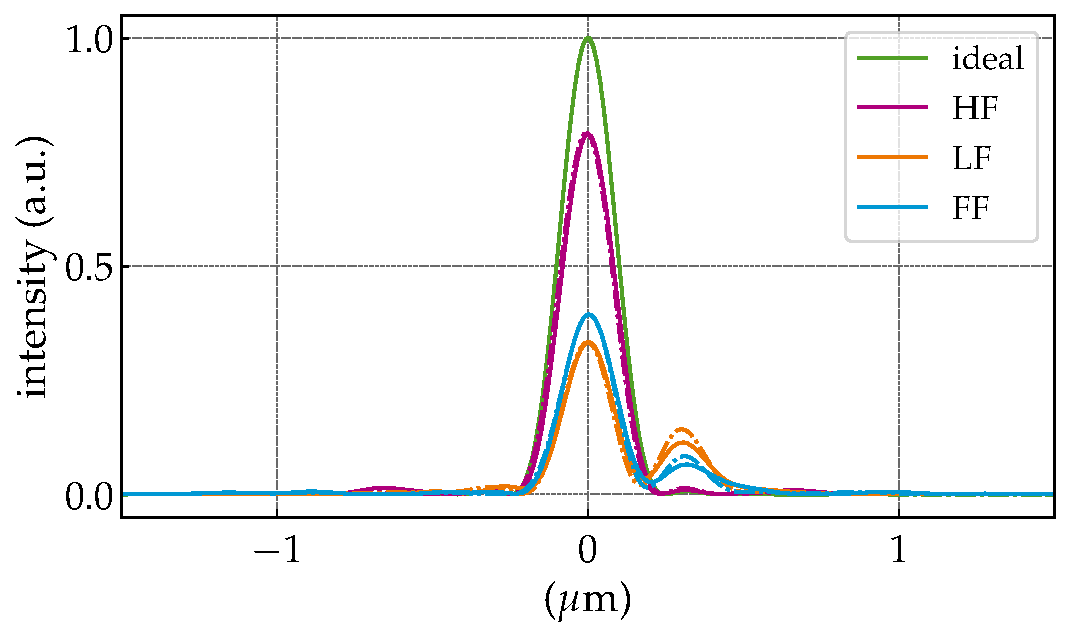
\includegraphics[height=3.3cm]{figures/ch05/CDnFF_LF_HH/Strehl_CDnFF_LF_HH.pdf}}
\end{figure}
\end{document}